\selectlanguage{ngerman}%
\frenchspacing%
\begin{ledgroupsized}[r]{120mm}%
\footnotesize%
\pstart%
\noindent\textbf{Überlieferung:}%
\pend%
\end{ledgroupsized}%
\begin{ledgroupsized}[r]{114mm}%
\footnotesize%
\pstart%
\parindent -6mm%
\makebox[6mm][l]{\textit{L}}%
Aufzeichnung:
LH XXXVII 4, Bl.\,157--158.
Ein Bogen 4\textsuperscript{o};
\href{\Scan{LH_37_04_157-158_wz}}{Wasserzeichen} mittig; %
Ränder beschnitten;
Papiererhltungsmaßnahmen.
Vier ganzseitig beschriebene Seiten.
\pend%
\end{ledgroupsized}%
\selectlanguage{latin}%
\frenchspacing%
\vspace{5mm}%
\normalsize%
\pstart%
\noindent%
\lbrack%
\href{\Scan{LH_37_04_157r}}%
{157\,r\textsuperscript{o}}%
\rbrack%
\phantom{12 November 1677}%
\hfill%
\phantom{\lbrack157\,r\textsuperscript{o}\rbrack}%
12 Novembris 1677%
\pend%
\pstart%
\noindent%
\centering%
De Barometro portabili%
\indexS{barometrum portabile}%
\\
Scheda I%
\indexS{scheda}
\pend%
\vspace{0.5em}%
\pstart%
\noindent%
Barometrum portabile%
\indexS{barometrum portabile}
haberi potest,
si Thermometro%
\indexS{thermometrum portabile}
\edtext{%
conjungatur.%
\indexS{barometrum conjunctum thermometro}%
\indexS{thermometrum conjunctum barometro}
Sint%
}{%
\lemma{conjungatur.}%
\Bfootnote{%
\textit{(1)}~Sit %
\textit{(2)}~Sint%
~\textit{L}%
}}
Thermometrum \textit{ABC},%
\indexS{thermometrum portabile}
Barometrum \textit{DEF}%
\indexS{barometrum portabile}
inter se
\edtext{%
juncta %
per Tubulum \textit{CD}.%
\indexS{tubulus jungens barometrum et thermometrum}
Thermometrum \textit{ABC}%
\indexS{thermometrum portabile}
est sipho vitreus bicrurus%
\indexS{sipho bicrurus}%
\indexS{sipho vitreus}
in%
}{%
\lemma{juncta}%
\Bfootnote{%
\textit{(1)}~, id est %
\textit{(2)}~per Tubulum \textit{CD}. Thermometrum %
\textit{(a)}~compositum ex siphone %
\textit{(b)}~\textit{ABC} est sipho %
\bars{vitreus \textit{erg.}} bicrurus %
\textit{(aa)}~ex %
\textit{(bb)}~in%
~\textit{L}%
}}
duas pilas \textit{A} %
et \textit{C}%
\indexS{pila thermometri}
\edtext{%
desinens.
Barometrum \textit{DEF}%
\indexS{barometrum portabile}
est Tubus \textit{DE},%
\indexS{tubus recurvatus}
cui%
}{%
\lemma{desinens.}%
\Bfootnote{%
\textit{(1)}~Thermometrum est tubus \textit{DEF}, cui %
\textit{(2)}~Barometrum \textit{DEF} %
\lbrack...\rbrack\ \textit{DE}, cui%
~\textit{L}%
}}
insistit pila \textit{D},%
\indexS{pila barometri}
recurvatus in \textit{EF}.%
\indexS{tubus recurvatus}
Pila \textit{A}
habet Tubulum \textit{AH},
pila \textit{C}%
\indexS{pila thermometri}
tubulum \textit{CG},
et pila \textit{D}%
\indexS{pila barometri}
tubulum
\edtext{%
\textit{DG}.
Tubus \textit{AB} et tubus \textit{CB} %
separatim conflati
jungi possunt in
\lbrack\textit{B}\rbrack.%
\indexS{tubi juncti in thermometro}
Et similiter totum Thermometrum \textit{ABC}%
\indexS{barometrum conjunctum thermometro}%
\indexS{thermometrum conjunctum barometro}
jungi potest Barometro \textit{DEF}
mediantibus Tubulis%
\indexS{tubulus jungens barometrum et thermometrum}
\textit{CG}, \textit{DG}.%
}{%
\lemma{\textit{DG}.}%
\Bfootnote{%
\textit{(1)}~Unumquodque separatim fieri potest, %
\textit{(2)}~Tubus \textit{AB} %
\lbrack...\rbrack\ \textit{CB}, separatim %
\textit{(a)}~facti jungi %
\textit{(b)}~conflati jungi possunt in %
\bars{\textit{C} \textit{ändert Hrsg.}}. Et %
\textit{(aa)}~totum %
\textit{(bb)}~similiter totum Thermometrum \textit{ABC} %
\textit{(aaa)}~, tubulo \textit{CG}, %
\textit{(bbb)}~, median %
\textit{(ccc)}~jungi potest %
\textit{(aaaa)}~tubulo \textit{GD}, %
\textit{(bbbb)}~Barometri %
\textit{(cccc)}~Barometro \textit{DEF} %
\lbrack...\rbrack\ \textit{CG}, \textit{DG}.%
~\textit{L}%
}}
Nihil refert
quae sit altitudo,
crassities,
rectitudo tuborum %
ac pilarum.%
\edlabel{LH_37_04_157-158_157r_lor-1}%
\edtext{}{%
\xxref{LH_37_04_157-158_157r_lor-1}{LH_37_04_157-158_157r_lor-2}%
\lemma{pilarum.}%
\Bfootnote{%
\lbrack/\rbrack\
\textit{(1)}~Usus hic erit %
\textit{(2)}~His ita %
\lbrack...\rbrack\ ita praeparabitur:%
~\textit{L}%
}}%
\pend%
\begin{edfigure}[1.75em][0.0em]%
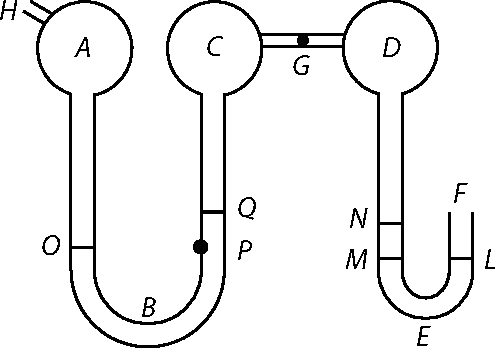
\includegraphics[width=0.45\textwidth]{gesamttex/edit_VIII-4/images/LH_37_04_157-158_d_157r.pdf}
\edcaption[-0.25em]%
{%
\hspace*{8mm}%
\lbrack\textit{Fig.\:1}\rbrack%
}%
\end{edfigure}%
\newpage%
\pstart%
His ita habitis,
instrumentum ita praeparabitur:%
\indexS{instrumentum portabile}%
\indexS{praeparatio thermometri}%
\indexS{praeparatio barometri}%
\edlabel{LH_37_04_157-158_157r_lor-2}
pilae%
\indexS{pila barometri}%
\indexS{pila thermometri}
\textit{C}, \textit{D}
\edtext{%
fortiter calefiant,%
\indexS{pila calefacta}%
}{%
\lemma{fortiter}%
\Bfootnote{%
\bars{et aequaliter \textit{gestr.}} calefiant,%
~\textit{L}%
}}
exibit aer per%
\indexS{exitus aeris e pila calefacta}%
\indexS{aer exiens e pila calefacta}
\edtext{%
\textit{F} et \textit{H}.%
}{%
\lemma{\textit{F} et}%
\Bfootnote{%
\textit{(1)}~\textit{A} %
\textit{(2)}~\textit{H}%
~\textit{L}%
}}
Quo facto%
\lbrack,\rbrack\
durante adhuc calore,%
\indexS{calor externus}
infundatur Mercurius utrinque,%
\indexS{mercurius infusus thermometro}%
\indexS{mercurius infusus barometro}
hinc per \textit{F},
\edtext{%
illinc per
\lbrack\textit{H}\rbrack.
Infusus%
\indexS{mercurius infusus barometro}
per \textit{F}
erit \textit{LEMN},
et \textit{MN}
refrigeratis tubis%
\indexS{tubus refrigeratus}
eminebit%
}{%
\lemma{illinc per}%
\Bfootnote{%
\bars{\textit{A} \textit{ändert Hrsg.}}. Infusus per \textit{F} %
\textit{(1)}~sit %
\textit{(2)}~erit \textit{LEMN}, %
\textit{(a)}~ita, ut %
\textit{(b)}~et \textit{MN} %
\bars{refrigeratis tubis \textit{erg.}} eminebit%
~\textit{L}%
}}
ultra horizontem \textit{LM}.%
\indexS{horizon}
Infusus%
\indexS{mercurius infusus thermometro}
\edtext{%
per \textit{H}%
}{%
\lemma{per}%
\Bfootnote{%
\textit{(1)}~\textit{A} %
\textit{(2)}~\textit{H}%
~\textit{L}%
}}
erit \textit{OPQ}.
His positis
ajo altitudinem%
\indexS{altitudo mercurii super horizontem}
\textit{PQ} aequalem
necessario esse altitudini%
\indexS{altitudo mercurii super horizontem}
\textit{MN},
quamvis tubi %
\textit{CB} et \textit{DE},%
\indexS{tubus recurvatus}
pilae \textit{C} et \textit{D},%
\indexS{pila barometri}%
\indexS{pila thermometri}
et quantitates infusi Mercurii%
\indexS{mercurius infusus thermometro}%
\indexS{mercurius infusus barometro}
\textit{OBP},
\textit{LEM} %
differant.
Nam ob communicationem pilarum%
\indexS{communicatio pilarum}
\textit{C} et \textit{D} in \textit{G}
aequaliter per eas distribuetur aer,%
\indexS{aer distributus in barometro}%
\indexS{aer distributus in thermometro}%
\indexS{distributio aeris in barometro}%
\indexS{distributio aeris in thermometro}
et %
utrobique
\edtext{%
tam per \textit{H} %
quam%
}{%
\lemma{tam}%
\Bfootnote{%
\textit{(1)}~per \textit{A} %
\textit{(a)}~q %
\textit{(b)}~\textlangle\textendash\textrangle\ %
\textit{(2)}~per \textit{H} %
quam%
~\textit{L}%
}}
per \textit{F} %
aequalis vis premit,%
\indexS{vis aeris prementis}%
\indexS{aer premens}%
\indexS{pressio aeris}
pondus scilicet aeris%
\indexS{pondus aeris}
\edtext{%
cujus effectus in liquore%
\indexS{liquor in barometro}%
\indexS{liquor in thermometro}%
\indexS{effectus ponderis aeris in liquore}%
}{%
\lemma{cujus}%
\Bfootnote{%
\textit{(1)}~in liquore %
\textit{(2)}~effectus in liquore%
~\textit{L}%
}}
tantum secundum altitudinem%
\indexS{altitudo mercurii super horizontem}
qua super horizontem eminet,%
\indexS{horizon}
utrinque spectari potest.
Cum ergo eadem utrinque vis%
\indexS{vis aeris prementis}
et resistentia sit,%
\indexS{resistentia ad pressionem aeris}
idem utrobique effectus%
\indexS{effectus ponderis aeris in liquore}%
\lbrack,\rbrack\
scilicet Mercurii altitudo erit.%
\indexS{altitudo mercurii super horizontem}
\edtext{%
Jam Tubulum \textit{H} hermetice sigillabimus,%
\indexS{tubulus hermetice sigillatus}
et tubulum \textit{CGD}
flatu molliendo%
\indexS{flatus}
in medio \textit{G}
\lbrack di\rbrack ducemus,
diductis a se invicem
Thermometro \textit{ABC}%
\indexS{thermometrum portabile}
et Barometro \textit{DEL},%
\indexS{barometrum portabile}
donec diversis sigillationibus%
\indexS{sigillatio}
separare eos %
et relictum in medio inter eas
impune abrumpere liceat.%
}{%
\lemma{Jam}%
\Bfootnote{%
\textit{(1)}~Jam duo instrumenta %
\textit{(2)}~\bars{Jam \textit{streicht Hrsg.}} %
\textit{(a)}~Barometrum a Thermometro separabimus %
\textit{(b)}~Tubulum \textit{H} hermetice %
\lbrack...\rbrack\ in medio \textit{G} %
\bars{ducemus \textit{ändert Hrsg.}}, diductis a se invicem %
\textit{(aa)}~hinc Barometro %
\textit{(bb)}~Thermometro \textit{ABC} %
\lbrack...\rbrack\ \textit{DEL}, donec %
\textit{(aaa)}~amborum extremi %
\textit{(bbb)}~diversis sigillationibus %
\lbrack...\rbrack\ in medio %
\bars{inter eas \textit{erg.}} impune abrumpere liceat.%
~\textit{L}%
}}
Cavendum tantum
ut durante
\lbrack%
\href{\Scan{LH_37_04_157v}}%
{157\,v\textsuperscript{o}}%
\rbrack\
flatu%
\indexS{flatus}
isto novissimo
non plus una pila%
\indexS{pila barometri}%
\indexS{pila thermometri}
quam alia
\edtext{%
calefiat%
\indexS{pila calefacta}%
\lbrack;\rbrack\
quod%
}{%
\lemma{calefiat~,}%
\Bfootnote{%
\textit{(1)}~quod %
\textit{(2)}~ne %
\textit{(3)}~quod%
~\textit{L}%
}}
facile caveri potest.
Ambae enim in loco sunt aeque calido,
et flatus%
\indexS{flatus}
non ipsas
sed medium commissurae \textit{G}%
\indexS{commissura barometri et thermometri}
attingit%
\lbrack,\rbrack\
\edtext{%
idque facile est dignoscere,
quia %
statim videri potest %
an eadem maneat altitudo \textit{MN} et \textit{PQ}.%
\indexS{altitudo mercurii super horizontem}%
}{%
\lemma{idque facile %
\lbrack...\rbrack\ potest an}%
\Bfootnote{%
\textit{(1)}~eandem altitudinem %
\textit{(2)}~eadem %
\textit{(a)}~altitudo %
\textit{(b)} maneat altitudo \textit{MN} et \textit{PQ} %
\textit{erg.\;L}%
}}
Hoc posito
\edtext{%
et facta separatione%
\indexS{separatio barometri et thermometri}%
}{%
\lemma{et facta separatione}%
\Bfootnote{%
\textit{erg.\;L}%
}}
sequitur
eandem esse vim%
\indexS{vis aeris in pila}
seu consistentiam%
\indexS{consistentia aeris in pila}%
\indexS{aer in pila}
\edtext{%
aeris in pila \textit{C}%
\indexS{pila barometri}%
\indexS{pila thermometri}%
}{%
\lemma{aeris in}%
\Bfootnote{%
\textit{(1)}~medio %
\textit{(2)}~pila \textit{C}%
~\textit{L}%
}}
Thermometri%
\indexS{thermometrum portabile}
et in pila \textit{D} Barometri,%
\indexS{barometrum portabile}
unde gradus Thermometri%
\indexS{thermometrum portabile}%
\indexS{gradus thermometri}
infra vel supra
\edtext{%
statum communem%
\indexS{status communis atmosphaerae}
tempore elaborationis%
\indexS{tempus elaborationis}%
\indexS{elaboratio}%
}{%
\lemma{statum}%
\Bfootnote{%
\textit{(1)}~in quo tem %
\textit{(2)}~communem tempore %
\bars{primae \textit{gestr.}} elaborationis%
~\textit{L}%
}}
deprehensum reperti,
Barometro addentur%
\indexS{barometrum portabile}
vel
\edtext{%
detrahentur,
quia omnes effectus Thermometri%
\indexS{thermometrum portabile}%
\indexS{effectus thermometri repertus in barometro}
etiam%
}{%
\lemma{detrahentur,}%
\Bfootnote{%
\textit{(1)}~et ita %
\textit{(2)}~quia omnes
\textit{(a)}~impressiones Thermometri et %
\textit{(b)}~effectus Thermometri etiam%
~\textit{L}%
}}
in Barometro reperiuntur,
sed non contra.
Et cum in Barometro%
\indexS{barometrum portabile}
\edtext{%
distingui nequeant,%
}{%
\lemma{distingui}%
\Bfootnote{%
\textit{(1)}~nesciant %
\textit{(2)}~nequeant%
~\textit{L}%
}}
ope Thermometri adjecti%
\indexS{thermometrum adjectum barometro}
sine ullo calculo
accurate discernentur.
Quodsi Barometrum%
\indexS{barometrum portabile}
et Thermometrum%
\indexS{thermometrum portabile}
\edtext{%
hoc%
}{%
\lemma{hoc}%
\Bfootnote{%
\textit{erg.\;L}%
}}
non essent uno eodemque actu%
\indexS{actus}
elaborata,
calculo subtili%
\indexS{calculus subtilis}
quidem et certo,%
\indexS{calculus certus}
satis tamen perplexo%
\indexS{calculus perplexus}
opus foret.
\pend%
\newpage%
\pstart%
Utile erit
pilas esse%
\indexS{pila thermometri}%
\indexS{pila barometri}
quantum in portabili instrumento%
\indexS{instrumentum portabile}
commode licet
magnas.
Ita enim aer%
\indexS{aer nascens e mercurio}
ex Mercurio
tractu temporis%
\indexS{tractus temporis}%
\indexS{tempus}
nascens,%
\indexS{aer nascens e mercurio}
\edtext{%
nullam cum%
}{%
\lemma{nullam}%
\Bfootnote{%
\textit{(1)}~ad %
\textit{(2)}~cum%
~\textit{L}%
}}
pilarum magnitudine
comparationem
\edtext{%
habebit;
optimum autem erit%
}{%
\lemma{habebit;}%
\Bfootnote{%
\textit{(1)}~utile erit autem 
\textit{(2)}~optimum autem erit%
~\textit{L}%
}}
adhibere Mercurium%
\indexS{mercurius purgatus aere}
qui jam sit ab aere purgatus.%
\indexS{mercurius purgatus aere}
\pend%
\pstart%
Porro
ut in exiguo
\edtext{%
\lbrack quantum\rbrack%
}{%
\lemma{quantum}%
\Bfootnote{%
\textit{erg.\;Hrsg.}%
}}
licet instrumento%
\indexS{instrumentum portabile}
quod tubum calamarium non excedat%
\indexS{tubus calamarius}
omnes effectus exhibeantur%
\indexS{effectus exhibitus in instrumento}
satis
\edtext{%
distincte%
\lbrack,\rbrack\
regula%
\indexS{regula divisa exacte}%
\indexS{regula applicata instrumento}
applicari potest %
exactissime divisa
vel%
}{%
\lemma{distincte;}%
\Bfootnote{%
\textit{(1)}~vel %
\textit{(2)}~regula applicari %
\lbrack...\rbrack\ divisa vel%
~\textit{L}%
}}
punctis vel filis tenuissimis circumligatis,
sed necesse erit
instrumentum directe statui horizontale.%
\indexS{instrumentum portabile}
In Barometro%
\indexS{barometrum portabile}
poterimus adhibere
\edtext{%
pondus%
\indexS{pondus innatans mercurio}
Mercurio \textit{F} innatans%
}{%
\lemma{pondus}%
\Bfootnote{%
\textit{(1)}~in \textit{F} %
\textit{(2)}~Mercurio \textit{F} innatans%
~\textit{L}%
}}
\edlabel{LH_37_04_157-158_157v_udz-1}%
ut
\edtext{%
in Barometris Anglicanis,%
\indexS{barometrum Anglicanum}%
\edlabel{LH_37_04_157-158_157v_udz-2}%
}{%
\lemma{in Barometris Anglicanis}%
\Cfootnote{%
Wohl Anspielung auf das von Hooke erfundene Radbarometer,
welches für die Betätigung des Zeigers die Anwendung eines im Quecksilber schwimmenden Körpers vorsah.
Siehe \textsc{R.\;Hooke},
\textit{Micrographia}, Preface
(London 1665, S.\:[c3] u.\;Tafel I, Abb.\;I);%
\cite{00061}
\textsc{Ders.},
\glqq A new Contrivance of Wheel-Barometer\grqq\
(\textit{PT}, I, 4.\;Juni 1666,
S.\;218\,f. u.\;Abb.\;1 vor S.\;215).%
\cite{01523}
Auf das \glqq englische\grqq\ Radbarometer beziehen sich in diesem Band auch die Aufzeichnung
N.\;\ref{57041}
(\refpassage{LH_37_04_162-163_163r_hooke-1}{LH_37_04_162-163_163r_hooke-2}
u.\;\refpassageohne{LH_37_04_162-163_163r_hooke-3}{LH_37_04_162-163_163r_hooke-4})
vom Oktober 1677
sowie die spätere Aufzeichnung
N.\;\ref{53451}
(\refpassage{LH_37_04_171_171r_hooke-1}{LH_37_04_171_171r_hooke-2}).%
}}
\lbrack%
\href{\Scan{LH_37_04_158r}}%
{158\,r\textsuperscript{o}}%
\rbrack\
quod artificium%
\indexS{artificium applicatum barometro}
si ad Thermometrum hoc clausum%
\indexS{thermometrum clausum}
sed exiguum et portabile%
\indexS{thermometrum portabile}
applicare vellemus,
opus esset
in Thermometro natare frustum ferri%
\indexS{ferrum}%
\indexS{frustum ferri in thermometro}
aut magnetis%
\indexS{magnes}%
\indexS{frustum magnetis in thermometro}
in \textit{Q},
quod applicatum extra %
\edtext{%
aliud frustum%
}{%
\lemma{aliud}%
\Bfootnote{%
\textit{(1)}~frustra %
\textit{(2)}~frustum%
~\textit{L}%
}}
magnetis%
\indexS{magnes}%
\indexS{frustum magnetis in thermometro}
aut ferri%
\indexS{ferrum}%
\indexS{frustum ferri in thermometro}
secum attollat deprimatque.
Quo
\edtext{%
facto
illud quoque facili machinatione%
\indexS{machinatio}%
}{%
\lemma{facto}%
\Bfootnote{%
\textit{(1)}~statim %
\textit{(2)}~illud quoque facili machinatione%
~\textit{L}%
}}
efficere licebit,
ut gradus Thermometri%
\indexS{thermometrum portabile}%
\indexS{gradus thermometri}
sese ipsi a Barometro%
\indexS{barometrum portabile}%
\indexS{gradus barometri}
detrahant,
nec ullo calculo%
\indexS{calculus}
opus sit.
Ita Barometrum hoc%
\indexS{barometrum portabile}
in marsupio gestatum,%
\indexS{marsupium}%
\indexS{barometrum gestatum in marsupio}
aut in hypocausta%
\indexS{hypocaustum}%
\indexS{barometrum translatum in hypocaustum}
ac balnea%
\indexS{balneum}%
\indexS{barometrum translatum in balneum}
translatum%
\lbrack,\rbrack\
nullam subibit mutationem.%
\indexS{mutatio barometri}
\pend%
\pstart%
Porro eundem effectum%
\indexS{effectus assecutus ope duorum barometrorum}
forte etiam ope duorum Barometrorum%
\indexS{barometrum portabile}
sed diversae pilarum%
\indexS{pila barometri}
rationis %
assequi licebit,%
\indexS{effectus assecutus ope duorum barometrorum}
atque ita carere licebit magnete.%
\indexS{magnes}
Ponamus enim
aerem unius pilae%
\indexS{aer in pila}
esse rariorem%
\indexS{aer rarus}
quam aerem alterius pilae,%
\indexS{pila barometri}
quod qua proportione fiat
discere licebit ex ratione ipsius \textit{NM}
altitudinis Mercurii super horizontem%
\indexS{altitudo mercurii super horizontem}%
\indexS{horizon}
\edtext{%
in uno tubo,%
\indexS{tubus recurvatus}
ad \textit{PQ}%
}{%
\lemma{in}%
\Bfootnote{%
\textit{(1)}~una %
\textit{(2)}~uno tubo, ad %
\textit{(a)}~\textit{(N)(N)} %
\textit{(b)}~\textit{PQ} %
\textit{(c)}~\textit{PQ}%
~\textit{L}%
}}
altitudinem ejusdem in alio,
ponendo \textit{CQPBO} esse unum Barometrum%
\indexS{barometrum portabile}
(resecto \textit{OA})
et \textit{DNMEL} alterum.
Nimirum
\edtext{%
vis elastica%
\indexS{vis aeris elastica}
seu densitas aeris%
\indexS{densitas aeris}%
}{%
\lemma{vis}%
\Bfootnote{%
\textit{(1)}~aeris seu densitas %
\textit{(2)}~elastica seu densitas aeris%
~\textit{L}%
}}
in \textit{C},
juncta ponderi Mercurii \textit{QP},%
\indexS{pondus mercurii in thermometro}
est aequalis
\edtext{%
vi elasticae%
\indexS{vis aeris elastica}
seu densitati aeris%
\indexS{densitas aeris}%
}{%
\lemma{vi}%
\Bfootnote{%
\textit{(1)}~aeris %
\textit{(2)}~elasticae seu densitati aeris%
~\textit{L}%
}}
in \textit{D},
junctae ponderi mercurii \textit{NM}.%
\indexS{pondus mercurii in barometro}%
\edlabel{LH_37_04_157-158_158r_fsd-1}%
\edtext{}{%
\xxref{LH_37_04_157-158_158r_fsd-1}{LH_37_04_157-158_158r_fsd-2}%
\lemma{\textit{NM}.}%
\Bfootnote{%
\lbrack/\rbrack\ %
\textit{(1)}~Vis elastica a %
\textit{(2)}~Densitas aeris%
~\textit{L}%
}}%
\pend%
\newpage%
\pstart%
Densitas aeris%
\indexS{densitas aeris}%
\edlabel{LH_37_04_157-158_158r_fsd-2}
in \textit{C} %
vocetur \textit{d},
densitas ejusdem%
\indexS{densitas aeris}
in \textit{D}
vocetur $\delta$,
pondus Mercurii \textit{QP}%
\indexS{pondus mercurii in thermometro}
vocetur \textit{p},
et pondus Mercurii \textit{NM}%
\indexS{pondus mercurii in barometro}
vocetur $\pi$.
Ergo $d + p$ aequ.
\edtext{%
$\delta + \pi$ aequal. ipsi \textit{v}%
}{%
\lemma{$\delta + \pi$}%
\Bfootnote{%
\textit{(1)}~aequ. \textit{v} %
\textit{(2)}~aequal. ipsi \textit{v}%
~\textit{L}%
}}
ponderi
\edtext{%
praesenti%
}{%
\lemma{praesenti}%
\Bfootnote{%
\textit{erg.\;L}%
}}
totius Atmosphaerae,%
\indexS{pondus atmosphaerae}%
\indexS{atmosphaera}
\edtext{%
seu ponderi Mercurii
cujus altitudo 27%
\indexS{pondus mercurii 27 pollicum}
vel 30 pollicum;%
\indexS{pondus mercurii 30 pollicum}%
\indexS{pollex}%
}{%
\lemma{seu}%
\Bfootnote{%
\textit{(1)}~ponderi praesenti %
\textit{(2)}~ponderi Mercurii cujus altitudo %
\textit{(a)}~30 pollicum %
\textit{(b)}~27 vel 30 pollicum;%
~\textit{L}%
}}
nota autem altitudo \textit{QP} %
et \textit{NM},
ergo et ratio ejus ad pollices%
\indexS{pollex}
istos totius altitudinis,%
\indexS{altitudo mercurii super horizontem}
notae ergo potentiae%
\indexS{potentia aeris elastica}
\textit{p}, $\pi$
in ratione ad
\edtext{%
totam \textit{v}.
Et quia
\textit{d} aequ. $v - p$
et
$\delta$ aequ. $v - \pi$,%
}{%
\lemma{totam \textit{v}.}%
\Bfootnote{%
\textit{(1)}~Ergo quia datur %
\textit{(2)}~Et quia \textit{d} aequ. $v-p$ %
\textit{(a)}~et $\delta$ %
\textit{(b)}~et $\delta$ aequ. $v - \pi$,%
~\textit{L}%
}}
dabitur
$\dfrac{d}{\delta}$
\edtext{%
aequ.
$\dfrac{v-p}{v-\pi}$.%
}{%
\lemma{aequ.}%
\Bfootnote{%
\textit{(1)}~$\dfrac{v - \pi}{v - \hphantom{p}}$ %
\textit{(2)}~$\dfrac{v - p}{v - \pi}$%
~\textit{L}%
}}
Hinc aucta \textit{v},
\edtext{%
seu atmosphaerae pondere,%
\indexS{pondus atmosphaerae}%
\indexS{atmosphaera}
augentur
\lbrack%
\href{\Scan{LH_37_04_158v}}%
{158\,v\textsuperscript{o}}%
\rbrack\
\textit{p} et $\pi$ tantundem;%
}{%
\lemma{seu}%
\Bfootnote{%
\textit{(1)}~aeris p %
\textit{(2)}~atmosphaerae pondere, augentur %
\textit{(a)}~$\pi$ et %
\textit{(aa)}~\textlangle t\textrangle\ %
\textit{(bb)}~\textit{p} %
\lbrack\href{\Scan{LH_37_04_158v}}{158\,v\textsuperscript{o}}\rbrack\ %
\textit{(b)}~\textit{p} et $\pi$ tantundem;%
~\textit{L}%
}}
\rule[0mm]{0mm}{3.2mm}%
quia \textit{d} et $\delta$
ex hypothesi%
\indexS{hypothesis}
non augentur.
Porro calore externo%
\indexS{calor externus}
augentur
etiam \textit{d} et $\delta$,
quorum
cum ratio sit nota %
ante mutationem,%
\indexS{mutatio ponderis atmosphaerae}
videtur etiam
nota esse
post
\edtext{%
mutationem%
\indexS{mutatio ponderis atmosphaerae}%
\lbrack;\rbrack\
videtur enim
quo plenior seu densior est aer,%
\indexS{aer densus}
hoc majorem vim se dilatandi%
\indexS{vis aeris dilatandi se}
acquirere aequali calor\lbrack e\rbrack,%
\indexS{calor aequalis}
seu duorum aerum%
\indexS{aer calefactus}
eodem calore%
\indexS{calor externus}
quaesitas se dilatandi vires%
\indexS{vis aeris dilatandi se}%
}{%
\lemma{mutationem,}%
\Bfootnote{%
\textit{(1)}~quia semper %
\textit{(a)}~eat %
\textit{(b)}~propo %
\textit{(c)}~aer raref %
\textit{(2)}~videtur enim %
\lbrack...\rbrack\ aer, hoc %
\textit{(a)}~\textlangle neq\textrangle\ %
\textit{(b)}~majorem vim se dilatandi %
\textit{(aa)}~aequa %
\textit{(bb)}~acquirere aequali %
\bars{calores \textit{ändert Hrsg.}}, seu %
\textit{(aaa)}~duas vires elasticas duorum aerum dilatatorum%
\indexS{vis elastica aeris dilatati}\indexS{aer dilatatus} %
\textit{(bbb)}~duorum aerum %
\lbrack...\rbrack\ dilatandi vires%
~\textit{L}%
}}
esse in ratione \textit{d} ad $\delta$,
quo posito dabitur semper
$\dfrac{v - p}{v - \pi}$;%
\rule[0mm]{0mm}{6.0mm}
dantur autem \textit{p} et $\pi$,
ergo dabitur~\textit{v},
seu facta in pondere atmosphaerae mutatio,%
\indexS{mutatio ponderis atmosphaerae}%
\indexS{pondus atmosphaerae}%
\indexS{atmosphaera}
scilicet
quia datur $\dfrac{d}{\delta}$,
erit
$v\delta - p\delta$
aequ.
$vd - \pi d$.
Ergo
$vd - v\delta$
aequ.
$\pi d - pd$.%
\rule[0mm]{0mm}{5.8mm}
Ergo
$\dfrac{v}{\pi - p}$
aequ.
\edtext{%
$\dfrac{d}{d - \delta}$.
$\dfrac{d}{\delta}$ aequ. $\theta$.%
}{%
\lemma{$\dfrac{d}{d - \delta}$}%
\Bfootnote{%
\textit{(1)}~(seu $\dfrac{v}{p-\pi}$ aequ. $\dfrac{\delta}{\delta-d}$ seu $\dfrac{v}{\pi-p}$ aequ. $\dfrac{\delta}{d-\delta}$. Ergo $\dfrac{\delta}{d-\delta}$ aequ. $\dfrac {d}{d-\hphantom{d}}$ %
\textit{(2)}~. $\dfrac{d}{\delta}$ aequ. $\theta$.%
~\textit{L}%
}}
Ergo
$v - p$ aequ. $v\theta - \pi\theta$
seu
$v - v\theta$ aequ. $p - \pi\theta$
seu
\textit{v} aequ. $\dfrac{p - \pi\theta}{1 - \theta}$.%
\rule[0mm]{0mm}{6.0mm}
Est autem $1 - \theta$ quantitas constans,%
\indexS{quantitas constans}
quia $\theta$ est quantitas constans.%
\indexS{quantitas constans}%
\rule[0mm]{0mm}{5.8mm}
Porro ut res facilius peragatur instrumento,%
\indexS{instrumentum portabile}%
\indexS{res peracta instrumento}
sit \textit{p} aequ. $\beta + \pi$.
Ergo fiet
$\dfrac{\beta}{1 - \theta} + \pi$
\edtext{%
aequ.\;\textit{v},%
\rule[0mm]{0mm}{7.0mm}
nam si \textit{p} est major quam $\pi$,
est \textit{d} minor quam $\delta$,
seu 1 major quam $\dfrac{d}{\delta}$ vel $\theta$.%
}{%
\lemma{aequ.\;\textit{v}}%
\Bfootnote{%
\textit{(1)}~vel potius quia $\theta$ major unitate, %
\textit{(2)}~nam si %
\lbrack...\rbrack\ quam $\pi$, est %
\textit{(a)}~etiam %
\textit{(b)}~\textit{d} %
\textit{(aa)}~major %
\textit{(bb)}~minor quam $\delta$, %
\lbrack...\rbrack\ vel $\theta$.%
~\textit{L}%
}}
Arte ergo opus%
\indexS{ars}
\edtext{%
est qua%
}{%
\lemma{est}%
\Bfootnote{%
\textit{(1)}~per quam %
\textit{(2)}~qua%
~\textit{L}%
}}
in ipsa machina%
\indexS{machina}
dividatur $\beta$ per
\edtext{%
numerum%
}{%
\lemma{numerum}%
\Bfootnote{%
\textit{erg.\;L}%
}}
constantem%
\indexS{numerus constans}
\edtext{%
$1 - \theta$,
et productum ipsi $\pi$ addatur,%
}{%
\lemma{$1 - \theta$,}%
\Bfootnote{%
\textit{(1)}~quod per applicatam exiguam %
\textit{(2)}~et productum ipsi %
\textit{(3)}~et productum ipsi $\pi$ addatur,%
~\textit{L}%
}}
\ledpb%
id vero facile est,
\edtext{%
si in numeri istius ratione%
}{%
\lemma{si}%
\Bfootnote{%
\textit{(1)}~per numerum istum %
\textit{(2)}~in numeri istius ratione%
~\textit{L}%
}}
cylinder ille exiguus%
\indexS{cylinder}
cujus ope major circulus%
\indexS{circulus}
indici datur,
diminuatur,
et numerus
\edtext{%
graduum proveniens excentrice%
}{%
\lemma{graduum}%
\Bfootnote{%
\textit{(1)}~excentrice %
\textit{(2)}~proveniens excentrice%
~\textit{L}%
}}
alterius indicis gradus augeat,%
\indexS{gradus indicis}%
\indexS{index graduum mutationis atmosphaerae}
ita enim
quia eccentrice additur,
minus addetur,
quam si divisio facta non fuisset %
in ea quae desideratur ratione.
Quoniam tamen calculus hoc modo facillimus est,%
\indexS{calculus facillimus}
non opus est
ut huic rei immoremur.
Nimirum
quoniam numeri $\pi$ et $\beta$ statim visu apparent,
tantum monendi homines%
\indexS{homo}
paucis verbis machinae ascriptis,%
\indexS{machina}
quod per numerum illum constantem $(1 - \theta)$%
\indexS{numerus constans}
divisus numerus $\beta$
additus numero $\pi$
daturus sit \textit{v}.
\pend%
\selectlanguage{latin}%
\frenchspacing%
\normalsize%
